\documentclass[conference]{IEEEtran}
\IEEEoverridecommandlockouts
% The preceding line is only needed to identify funding in the first footnote. If that is unneeded, please comment it out.
\usepackage{cite}
\usepackage{blindtext}  % generate random text
\usepackage{amsmath,amssymb,amsfonts}
\usepackage{algorithm}
% \usepackage{algorithmic}
\usepackage{graphicx}
\usepackage{textcomp}
\usepackage{xcolor}
\usepackage{algpseudocode}
\usepackage{graphicx}
\usepackage{hyperref}

\def\BibTeX{{\rm B\kern-.05em{\sc i\kern-.025em b}\kern-.08em
    T\kern-.1667em\lower.7ex\hbox{E}\kern-.125emX}}
\begin{document}

\title{Matrix Transposition and Symmetry: a case study on Superscalar Architectures\\
%{\footnotesize \textsuperscript{*}Note: Sub-titles are not captured in Xplore and
%should not be used}
%\thanks{Identify applicable funding agency here. If none, delete this.}
}

\author{\IEEEauthorblockN{Giovanni Santini}
\IEEEauthorblockA{\textit{Dept.\ of Information Engineering and Computer Science} \\
\textit{University of Trento}\\
Trento, Italy \\
giovanni.santini@studenti.unitn.it \\
MAT. 235441}
}

\maketitle


\begin{abstract}
Contemporary CPU designs achieve higher performance by integrating multicore processing with sophisticated Single Instruction Multiple Data (SIMD) capabilities.
This study investigates the performance of two algorithms—square matrix transposition and symmetry checking—on modern superscalar CPU architectures. Both implicit and explicit parallelism techniques will be discussed, as well as the effects of compiler optimization flags.
\end{abstract}

\begin{IEEEkeywords}
parallel computing, matrix transpose, symmetric matrix, benchmark
\end{IEEEkeywords}

\section{Introduction}

Modern CPUs make use of superscalar architectures to improve performance, combining multiple cores with advanced Single Instruction Multiple Data (SIMD) technologies. Examples include Intel's Streaming SIMD Extensions (SSE) and Advanced Vector Extensions (AVX). Although SSE is not a new technology, being first introduced in the Pentium III in 1999 and subsequently expanded in later years \cite{b1}, modern algorithms leveraging SIMD instructions continue to be a topic of active research in recent literature.
For example, the FreeBSD's SIMD-enhanced libc is actively reworking the standard library's code. \cite{b2}.
In 2023, most of the string functions were reimplemented by Robert Clausecker et al on many architectures \cite{b3}, exploiting vector instructions and improving the overall performance of the standard library \cite{b4}.
Similarly, efficient multi-threaded algorithms are becoming more critical as the demand of computation increases worldwide due to AI training \cite{b5} \cite{b6}.
This case study examines the implementations and performance of two algorithms—out-of-place square matrix transposition (matTranspose) and square matrix symmetry checking (checkSymm)—in the context of a superscalar architecture. Both algorithms have been used pervasively in performance critical applications. For example, matrix transposition was used in NASA's Apollo 11 Guidance Computer (AGC) to convert vectors in platenary coordinate system to base reference system \cite{b7}. Additionally, matrix transposition is used by Fourier Transform in the West (FFTW) \cite{b8}, a popular library to calculate Fast Furier Transofrms, and in signal processing \cite{b9}. Furthermore, the current C++26 draft proposes basic linear algebra algorithms in the "linalg" header, including matrix transposition \cite{b10}.

In section 2, we discuss the state of the art of the two algorithms.
In section 3, we elaborate on the algorithms analyzed.
In section 4, we explain the benchmarking procedures and system information.
In section 5, we present the results. The conclusion is in section 6. Section 7 contains
the project's github link


\section{State of the Art}

\iffalse

\textit{We define the transpose of a matrix $A$, and we denote it by $A^t$, as the matrix obtained from $A$ by interchanging rows and columns. Specifically, if $A$ is an $m$-by-$n$ matrix, then $A^t$ is the $n$-by-$m$ matrix whose entries are given by the equation (1)}. \cite{b11}


\begin{equation}
	(A^t)_{k,j} = A_{j,k}
\end{equation}

\fi

Computing the transpose of a matrix is a well discussed computational problem. Early
work focuses on in-situ transporision, that is transposing a matrix without
relying on additional space. Implementations were often based on the cyclic
structure of the transposition mapping: values of a matrix of size $N$ can be stored
in a single contiguous array or size $N$*$N$ and indexed with $row*\#rows+ column$.
Remarcable contributions include Boothroyd's ACM Algorithm 302 (1966) using cyclic mapping \cite{b13}, Laflin and Brefner ACM Algorithm 380
adding fixed points arithmetic \cite{b14} and
a later revision of the two by Esko G. Cate and David W. Twigg in ACM Algorithm 513 \cite{b15} .
SIMD implementations for specific architectures are also widely adopted
in performance critical applications like cryptographic libraries, utilizing instructions like Intel's vpunpckldq and vpunpckhdq \cite{b16} and reporting improvements up to 70\% \cite{b17}.
However, vector registers are unoptimal for matrices since registers read data only sequencially, motivating research on new vector register file (VFS) designs such as diagonal registers \cite{b23}.
Another area of research includes out-of-core matrix transposition, that
is computing the transpose of a matrix that exceeds the size of the available in-core memory.
This problem focuses on optimizing the number of I/O operations and file layout since memory-memory data transfer is notably slower than math operations. Work in out-of-core transposition include W. 0. Alltop (1975) \cite{b18}, Suh \& Prasanna (2002) \cite{b19} and Krishnamoorth et al. (2004) \cite{b20}.
Recent work explores parallelization and the use of GPUs to offload algebra operations. Examples are I-Jui Sung et al \cite{b21} and Mark Harris \cite{b22}.

\iffalse
\textit{A square matrix $A$ is called symmetric if it equals its transpose} \cite{b12}.
\fi 
While symmetric matrces are actively used in various areas of research as their
properties allow for several optimizations in various problems, an in depth case study of symmetry
checking on modern architectures is yet to be published.

\section{Contribution and Methodology}

\iffalse % pseudocode
    \begin{algorithmic}[1]
      \Procedure{MyProcedure}{}
      % use \state and \textit{} for variables
      % use \text for text
      % use \gets for assignments
      % use \If \EndIf \Return \Else
      \EndProcedure
    \end{algorithmic}
\fi 

In this report different implementations of \textit{matTranspose}
and \textit{checkSymm} are benchmarked, comparing implicit and explicit parallelism
techniques. In particular, the benchmarks aim to indicate cache and SIMD performance differences,
speedup with multiple threads and the impact of compile flags optimizations. Data will be compared visually via graphs. All benchmarks
will be tested against every matrix size from $2^2$ to $2^{12}$, we will assume the size value is a multiple of 4 for ease of implementation.  \\
The algorithms for \textit{matTranspose} will now be explained.
Each algorithm takes a $N \times N$ input square matrix \textit{input}, a matrix of the same shape \textit{ouput}, and the size of the two matrices \textit{size}.
The analyzed algorithms are the following:
\begin{itemize}
\item \textit{matTranspose}: naive implementation of matTranspose, iterating over values of the input matrix and storing them in the output matrix with indexes of rows and columns swapped. See Algorithm~\ref{matTranspose} for the pseudocode.

\begin{algorithm}
	\caption{matTranspose}\label{matTranspose}
	\begin{algorithmic}[1]
		\For{\textit{r} \textbf{ in } \textit{0..size-1}}
	    \For{\textit{c} \textbf{ in } \textit{0..size-1}}
		\State $output[c][r] \gets input[r][c]$
		\EndFor
		\EndFor
	\end{algorithmic}
\end{algorithm}

    \item \textit{matTransposeColumns}: similar to \textit{matTranspose}, but iterating on the input matrix first by columns and then by rows.
  The purpose of this implementation is to test a different access pattern.

\iffalse
\begin{algorithm}
	\caption{matTransposeColumns}\label{matTransposeColumns}
\begin{algorithmic}[1]
	\For{\textit{r} \textbf{ in } \textit{0..size-1}}
	 \For{\textit{c} \textbf{ in } \textit{0..size-1}}
            \State $output[r][c] \gets input[c][r]$
            \EndFor
        \EndFor
\end{algorithmic}
\end{algorithm}
\fi

  \item \textit{matTransposeHalf}: similar to \textit{matTranspose}, but the algorithm
  iterates only on the upper half of the input matrix. For each
  pair $(i,j)$ of indices of rows and columns in the upper half of the input matrix $M$, with output matrix $O$, $O[i][j]=M[j][i]$ and $O[j][i] = M[i][j]$.
\iffalse
\begin{algorithm}
	\caption{matTransposeHalf}\label{matTransposeHalf}
\begin{algorithmic}[1]
	\For{\textit{r} \textbf{ in } \textit{0..size-1}}
           \For{\textit{c} \textbf{ in } \textit{r..size-1}}
            \State $output[r][c] \gets input[c][r]$
            \State $output[c][r] \gets input[r][c]$
            \EndFor
        \EndFor
\end{algorithmic}
\end{algorithm}
\fi
  
\item \textit{matTransposeCyclic}: implementation of \cite{b13}, storing the matrix as a contiguous one-dimensional array of size $N*N$. See Algorithm~\ref{matTransposeCyclic} for the pseudocode.
  \begin{algorithm}
  	\caption{matTransposeCyclic}\label{matTransposeCyclic}
  \begin{algorithmic}[1]

  	  \For{\textit{n} \textbf{ in } \textit{0..size*size-1}}
        \State $int\ \textit{i} \gets \frac{n}{size}$
        \State $int\ \textit{j} \gets n \mod N$
        \State $T[n] \gets M[size * j + i]$
        \EndFor
          \end{algorithmic}
  \end{algorithm}

\item \textit{matTransposeIntrinsic}: based on \textit{matrix\_transpose4x4} from the linux kernel \cite{b16}, revised to work for out-of-place float matrices on x86 architectures and implemented using intrinsics. \textit{transpose\_4x4\_f32\_intrinsic} transposes a 4 by 4 matrix using vector registers of 128 bits by doing the following steps: load 4 rows of 4 floats from the the input matrix, combine pairs of rows in an alternating pattern (interleaving), shuffle to get the transpose and store them in the output matrix. \textit{matTransposeIntrinsic} iterates over 4x4 blocks in the input matrix, calling \textit{transpose\_4x4\_f32\_intrinsic} and saving the computed transposed block in the output matrix with rows and columns swapped. See Algorithm~\ref{matTransposeIntrinsic} for the pseudocode.
  \begin{algorithm}
	\caption{matTransposeIntrinsic}\label{matTransposeIntrinsic}
	    \begin{algorithmic}[1]
	\iffalse

      \Procedure{transpose\_4x4\_f32\_intrinsic}{Matrix4x4 in, Matrix4x4 out}
    \State \textbf{comment} Load rows  
    \State \textbf{comment} unpack and interleave rows
    \State \textbf{comment} Shuffle to form transposed rows
    \State \textbf{comment} Store transposed rows
      \EndProcedure
      
      \fi

        \For{$int\ i = 0, i < size, i += 4$}
        \For{$int\ j = 0, j < size, j += 4$}
        \State $transpose\_4x4\_f32\_intrinsic(input[i][j],$
        \State $                               output[j][i])$
        \EndFor
        \EndFor

    \end{algorithmic}
    \end{algorithm}

\item \textit{matTransposeIntrinsicCyclic}: same as \textit{matTransposeIntrinsic} but the matrix is saved as a one dimensional array similarly to \textit{matTransposeCyclic}
\item \textit{matTransposeVectorization}: similar to \textit{matTranspose} but the outer loop is decorated with $\# pragma\ simd $
%\item matTranspose half vectorization:
\item \textit{matTransposeUnrollingOuter}: similar to \textit{matTranspose} but the outer loop is manually unrolled. See Algorithm~\ref{matTransposeUnrollingOuter} for the pseudocode.

  \begin{algorithm}
    \caption{matTransposeUnrollingOuter}\label{matTransposeUnrollingOuter}
    \begin{algorithmic}[1]
        \For{$int\ c = 0, i < size, i += 4$}
            \For{\textit{r} \textbf{ in } \textit{0..size-1}}
            \State $output[c][r] \gets input[r][c]$
            \State $output[c+1][r] \gets input[r][c+1]$
            \State $output[c+2][r] \gets input[r][c+2]$
            \State $output[c+3][r] \gets input[r][c+3]$
            \EndFor
        \EndFor
    \end{algorithmic}
  \end{algorithm}

\item \textit{matTransposeUnrollingInner}: same as \textit{matTransposeUnrollingOuter} but the inner for loop is manually unrolled

\iffalse
\item \textit{matTransposeHalfUnrollingOuter}: same as \textit{matTransposeHalf} but the outer for loop is manually unrolled

\item \textit{matTransposeHalfUnrollingInner}: same as \textit{matTransposeHalf} but the inner for loop is manually unrolled
\fi

\item \textit{matTransposeCyclicUnrolled}: same as \textit{matTransposeCyclic} but the for loop in manually unrolled
\iffalse
  \begin{algorithm}
    \caption{matTranspose cyclic unrolled}\label{matTransposeCyclicUnrolled}
    \begin{algorithmic}[1]
      \Procedure{matTransposeCyclicUnrolled}{$Matrix input, Matrix output, int size$}
        \For{\textit{n} \textbf{ in } \textit{0..size*size-1}}
        \State $T[n] \gets M[size * ((n+1) \mod size ) + (\frac{n}{size})]$
        \State $T[n+1] \gets M[size * ((n+1+1) \mod size ) + (\frac{n+1}{size})]$
        \State $T[n+2] \gets M[size * ((n+2+1) \mod size ) + (\frac{n+2}{size})]$
        \State $T[n+3] \gets M[size * ((n+3+1) \mod size ) + (\frac{n+3}{size})]$
        \EndFor
      \EndProcedure
    \end{algorithmic}
  \end{algorithm}
  \fi
\item \textit{matTransposeOmpX}: this set of algorithms are all derived from \textit{matTranspose} with the outer for loops parallelized using omp with the number of threads \textit{X} being a power of 2 from $2^1$ to $2^6$.

\item \textit{matTransposeOmpXCollapse}: similar to \textit{matTransposeOmpX} but the for loops are parellelized using \textit{collapse(2)}
  
\item \textit{matTransposeOmp16SchedX}: similar to \textit{matTransposeOmpX} with 16 threads using different schedule algorithms, namely: static, dynamic, guided.
\end{itemize}

The algorithms for \textit{checkSymm} will now be explained. Each algorithm take an $N \times N$ square matrix \textit{input}, a size \textit{size} and return true if the matrix is symmetrix, false otherwise.
The analyzed algorithms are the following:
\begin{itemize}
\item \textit{checkSymm}: naive implementation of checkSymm. It Iterates over the upper half of the matrix and testing if every value is equal to the symmetric value.
% See Algorithm~\ref{checkSymm} for the pseudocode.

\iffalse
  \begin{algorithm}
    \caption{checkSymm}\label{checkSymm}
    \begin{algorithmic}[1]
        \State $\textbf{bool}\ isSymm \gets true$
        \For{\textit{i} \textbf{ in } \textit{0..size-1}}
            \For{\textit{j} \textbf{ in } \textit{i..size-1}}
            	\If{$input[i][j] != input[j][i]$}
            	\State $isSymm \gets \textbf{false}$
            	\EndIf
        	\EndFor
        \EndFor
        \State \Return $isSymm$
    \end{algorithmic}
  \end{algorithm}
\fi

% \item \textit{checkSymColumns}:
  
  % \item \textit{checkSymVectorization}
\item \textit{checkSymmUnrolledOuter}: similar to \textit{checkSymm} but the outer loop is manually unrolled.

\iffalse
  \begin{algorithm}
    \caption{checkSymmUnrolledOuter}\label{checkSymmUnrolledOuter}
    \begin{algorithmic}[1]
      \Procedure{checkSymmUnrolledOuter}{$Matrix input, int size$}
        \State $isSymm = true$
        \For{\textit{i} \textbf{ in } \textit{0..size-1}}
            \For{\textit{j} \textbf{ in } \textit{i..size-1}}
            \If $input[i][j] != input[j][i]$
            \State $isSymm = false$
            \EndIf
            \If $input[i+1][j] != input[j][i+1]$
            \State $isSymm = false$
                        \EndIf
            \If $input[i+2][j] != input[j][i+2]$
            \State $isSymm = false$
                        \EndIf
            \If $input[i+3][j] != input[j][i+3]$
            \State $isSymm = false$
                        \EndIf
        \EndFor
        \EndFor
        \Return $isSymm$
      \EndProcedure
    \end{algorithmic}
  \end{algorithm}
\fi
  
\item \textit{checkSymmUnrollingInner}: similar to \textit{checkSymmUnrolledOuter} but the inner loop is manually unrolled instead of the outer loop.
\item \textit{checkSymmUnrollingOuterBranchless}: similar to \textit{checkSymmUnrollingOuter}, but 4 pairs of values are checked for equality with a single math formula. The formula performs a XOR on 4 pairs of values and their transpose, if any of those are different than 0 then the matrix is not symmetric. See Arlgoritm~\ref{checkSymmUnrollingOuterBranchless} for the pseudocode.


\begin{algorithm}
	\caption{checkSymmUnrollingOuterBranchless}\label{checkSymmUnrollingOuterBranchless}
	\begin{algorithmic}[1]
		\State $\textbf{bool}\ isSymm \gets true$
		\For{$int\ i = 0;\ i < size;\ i += 4$}
		\For{$int\ j = i;\ j < size;\ j++$}
		\State $isSymm \gets isSymm\ \& $
		\State $(((input[i][j] \oplus input[j][i]) \mid $
		\State $(input[i+1][j] \oplus input[j][i+1]) \mid $
		\State $(input[i+2][j] \oplus input[j][i+2]) \mid $
		\State $(input[i+3][j] \oplus input[j][i+3])) == 0)$
		\EndFor
		\EndFor
		\State \Return $isSymm$
	\end{algorithmic}
\end{algorithm}

\item \textit{checkSymOmpX}: similar to \textit{matTransposeOmpX} but based on \textit{checkSymm}. After each parallel section, a barrier is needed to synchronize the shared boolean output variable.
\item \textit{checkSymOmpXCollapse}: similar to \textit{checkSymmOmpX} bur the two loops are parallelized with collapse(2).
\item \textit{checkSymm16SchedX}: similar to \textit{matTranspose16SchedX} but based on \textit{matTranspose}.
\end{itemize}

\iffalse
Remember: write
- what you did (contribution): high level overview like "hey, i want to test different vectorization ond parallelization implementations"
- how you did it (methodology): we benchmarked algorithm A ... (all the pseudocodes). Whay we mesured

\fi

\section{Experiments and System Description}

\iffalse
- Detailed description of the computing system and platform. \\
- Relevant specifications or configurations (e.g., libraries
and programming toolchains). \\
- Description of the experimental setup, procedures, and
methodologies used in the project. \\
- Discussion on how experiments are designed to test the hypotheses
or achieve the objectives \\
\fi

\iffalse
The experiments were conducted on a cluster equipped with 64 Intel(R) Xeon(R) Gold 6140M CPU with 2.30GHz, 32K of L1d cache, 32K L1i cache, 1025K L2 cache, 25344K L3 cache with cache lines of 64 bits, 1 thread per core, 4GB of DDR4 RAM running Linux 3.10.
The algorithms were benchmarked using valFuzz \cite{b24}. The set of benchmarks were compiled using gcc-9.1.0 with flags "-fopenmp", "-fopenmp-simd", 4 set of benchmarks are compiled with either no optimizations, -O1, -O2 and "-O3 -Ofast -march=native".
To obtain results with statistical significance, each benchmark has been executed 100 times collecting the following data concerning wall-clock execution time: minimum, maximum, median, arithmetic mean, standard deviation, Q1, Q3.
To prevent interference between the benchmarks, the cache is cleared by initializing an array twice as big as the L3 cache size.
To ensure fair comparison, the same input matrix is provided to all algorithms.
The input matrix is initialized with an uniform random distribution of floats ranging from -1 to 1 generated using a Linear Congruential Generator (LGC) \cite{b25} with the parameters $a=1664525$, $c = 1013904223$, $m=2^{32}$ \cite{b26} and seed $1337$.
To save time, generation of random numbers is done at compile time using tenno-tl \cite{b27}. Additional algorithms and data structures were used from tenno-tl including ranges and arrays.
\fi

Experiments were conducted on a cluster with 64 Intel(R) Xeon(R) Gold 5220 CPUs (2.20GHz) featuring 32K L1d and L1i caches, 1025K L2 cache, 25344K L3 cache (64-bit cache lines), 1 thread per core, and 4GB RAM, running Linux 3.10. The algorithms were benchmarked using valFuzz \cite{b24}, with benchmarks compiled using gcc-9.1.0 and flags "-fopenmp", "-fopenmp-simd". Four benchmark sets were compiled with different optimization levels: none, -O1, -O2 and "-O3 -Ofast -march=native".

To ensure statistical significance, each benchmark was executed 100 times, recording wall-clock execution time statistics: minimum, maximum, median, mean, standard deviation, Q1, and Q3. Cache interference was minimized by clearing it before each run by writing to an array twice the L3 cache size. Input matrices, consistent across algorithms, were initialized with uniformly random floats (-1 to 1) generated via a Linear Congruential Generator (LCG) \cite{b25} with parameters a=1664525, c=1013904223, m=232 \cite{b26}, and seed 1337.

To expedite random number generation, values were precomputed at compile time using tenno-tl \cite{b27}. Additional tenno-tl features, such as ranges and arrays, were also employed.

\section{Results and Discussion}

\iffalse
- Presentation of results \\
- Analysis and interpretation in context \\
- Comparison with the state-of-the-art \\

cinquantamila grafici qui

Mamma mia ma quanto e' veloce sto asesmbly,
buu al compilatore che non ci azzecca per bene. 
Anche ciclico è nammerda, invece l'unrolling
è figo.
In generale abbiamo capito
cose ed il cluster è pazzesco e le differenze
sono notevoli, evviva i soldi.

Ok fatto un po' meglio:



\fi

\iffalse
The results are now presented, matTranspose will be analyzed first.
The roofline model in figure~\ref{fig:transpose_benchmarks} (d) shows that the base algorithm is memory bounded so improvement over accessing memory efficiently will be rewarded. Starting from the algorithms without any parallelism depicted in figure~\ref{fig:transpose_base}, we notice \textit{matTransposeCyclic} to be constantly
slower that the others, while \textit{matTransposeColumns} shows little to no difference compared to the base algorithm with the same compiler flags. The performance difference between the other algorithms increases as more aggressive compiler optimizations are enabled. \textit{checkSymmHalf} becomes slower than the base line with the same optimizations, when they are enabled. 
Taking into consideration implicit parallelism techniques in figure~\ref{fig:transpose_benchmarks} (a), the faster algorithm is \textit{matTransposeIntrinsicCyclic} from size smaller than $10^2$, getting surpassed by \textit{matTransposeIntrinsic} and \textit{matTransposeUnrollingOuter} in larger matrices. \textit{matTransposeCyclicUnrolled} is the slower for all sizes. Looking at explicit parallelism in figure-\ref{fig:transpose_benchmarks} (b), benchmarks with giher number of threads take more time than benchmarks with fewer threads until around size $10^2$ to $10^3$ where the trend is inverted. When analysing schedulers, static is slower for most matrix sixzes but all algorithms converge to about the same timing in the bigger input. 
\fi 


\begin{figure}[htb]
	\centering
	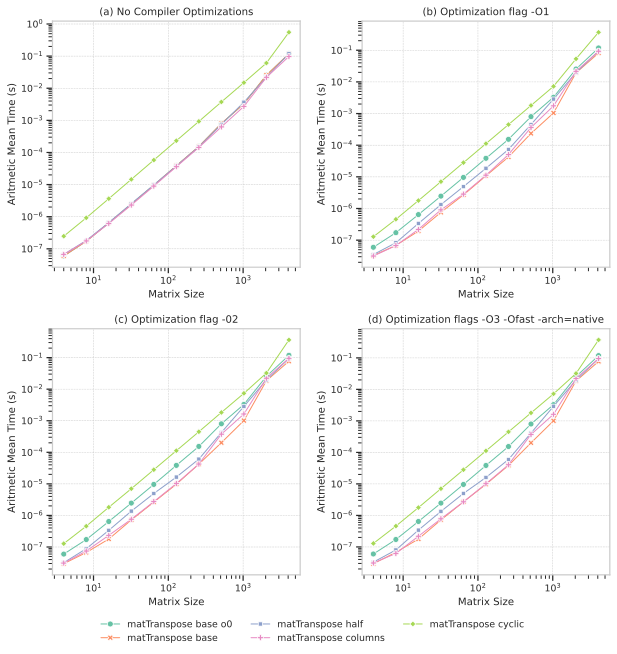
\includegraphics[width=0.45\textwidth]{"../benchmarks/plotting/images/transpose_base.pdf"}
	\caption{matTranspose results without parallelism}
	\label{fig:transpose_base}
\end{figure}
\begin{figure}[htb]
	
	\centering
	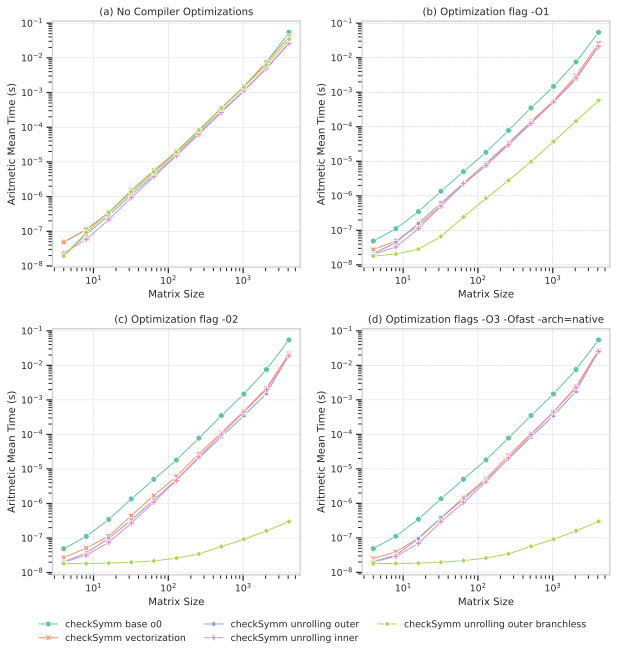
\includegraphics[width=0.45\textwidth]{"../benchmarks/plotting/images/symm_implicit.pdf"}
	\caption{checkSymm results with implicit parallelism}
	\label{fig:symm_implicit}
\end{figure}

\begin{figure}[htb]
	\centering
	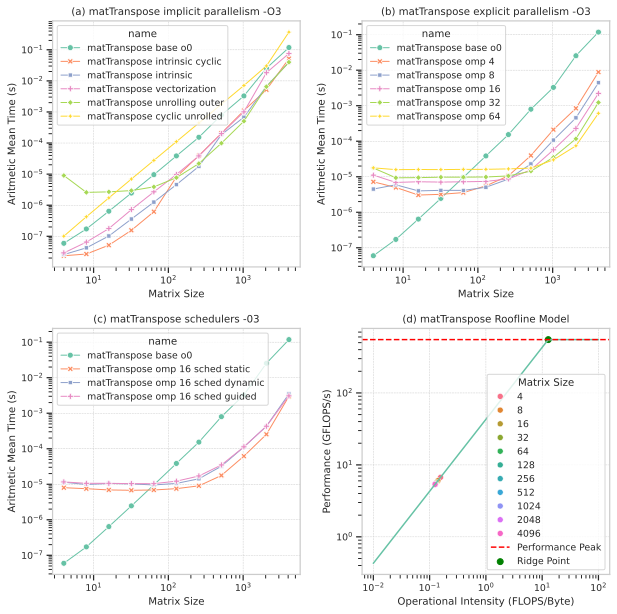
\includegraphics[width=0.45\textwidth]{"../benchmarks/plotting/images/transpose_all.pdf"}
	\caption{matTranspose results}
	\label{fig:transpose_benchmarks}
\end{figure}

\begin{figure}[htb]
	\centering
	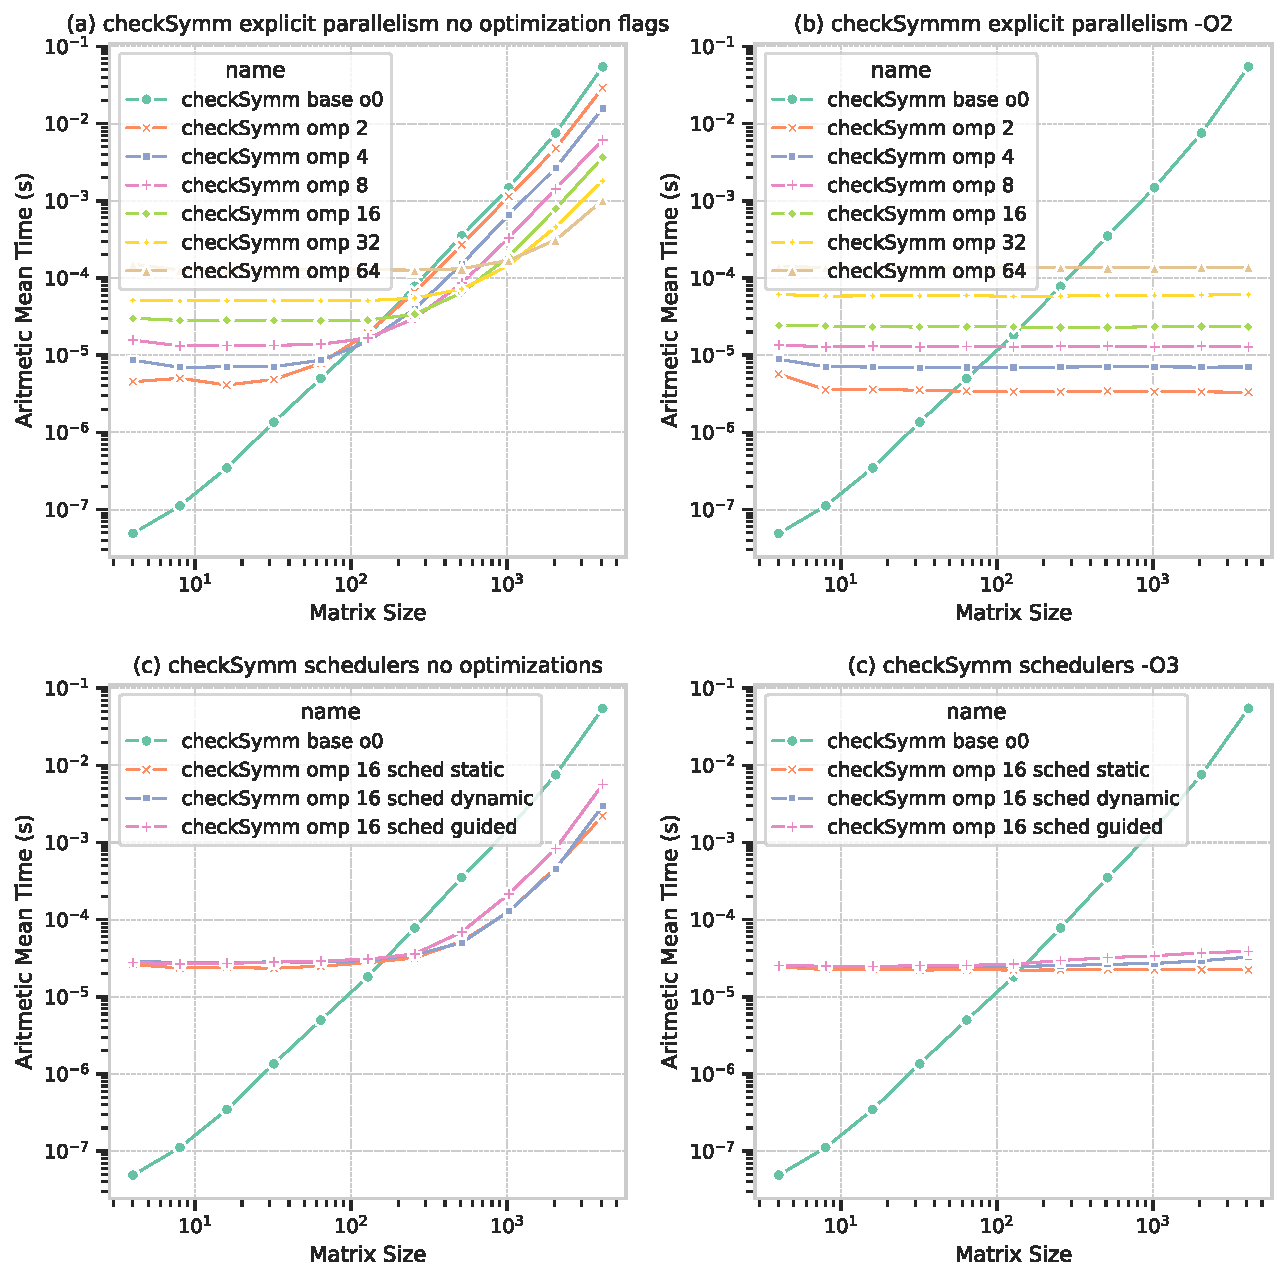
\includegraphics[width=0.45\textwidth]{"../benchmarks/plotting/images/symm_all.pdf"}
	\caption{checkSymm explicit parallelism results}
	\label{fig:symm_benchmarks}
\end{figure}

The results of the benchmarks are now presented, starting with \textit{matTranspose}.

% matTranspose

The roofline model of the base algorithm in Figure~\ref{fig:transpose_benchmarks}(d) indicates that the base algorithm is memory-bound, meaning improvements in memory access efficiency can significantly enhance performance. Among the non-parallel algorithms depicted in Figure~\ref{fig:transpose_base}, \textit{matTransposeCyclic} consistently underperforms compared to others. In contrast, \textit{matTransposeColumns} shows negligible difference relative to the base algorithm when identical compiler optimizations are applied. Notably, the performance gap among algorithms widens as more aggressive compiler optimizations are introduced. Interestingly, \textit{checkSymmHalf} becomes slower than the baseline when these optimizations are enabled.

When evaluating implicit parallelism techniques (Figure~\ref{fig:transpose_benchmarks}(a)), the fastest algorithm for matrices smaller than $10^2$ is \textit{matTransposeIntrinsicCyclic}. However, for larger matrices, \textit{matTransposeIntrinsic} and \textit{matTransposeUnrollingOuter} outperform it. Throughout all sizes, \textit{matTransposeCyclicUnrolled} remains the slowest.

Explicit parallelism results are illustrated in Figure~\ref{fig:transpose_benchmarks}(b). Benchmarks using a higher number of threads initially take longer to execute for matrices smaller than $10^3$. Beyond this range, the trend reverses, with higher-threaded configurations becoming more efficient. All parallel benchmarks after $10^2$ are faster than the base single-core algorithm. The results for \textit{matTransposeOmpXCollpase} show close similarity with the non collapsed version.

Finally, an analysis of scheduling (Figure~\ref{fig:transpose_benchmarks}(c)) shows that the static scheduler is generally slower for most matrix sizes. However, as matrix sizes increase, all algorithms converge to similar results.

% checkSymm

The results for \textit{checkSymm} are now presented. Among techniques utilizing implicit parallelism (Figure ~\ref{fig:symm_implicit}), there is minimal speed difference between methods, even with compiler optimizations enabled. The sole exception is \textit{checkSymmUnrollingOuterBranchless}, which significantly outperforms the others when optimizations are applied, leveraging SIMD instructions on the CPU for maximum efficiency.

Explicit parallelism results (Figure~\ref{fig:symm_benchmarks}) mirror those observed in \textit{matTranspose}, initially showing poorer performance with higher thread counts. This trend reverses between input sizes of $10^2$ and $10^3$ when no compiler optimizations are used. Interestingly, with optimizations enabled, execution time exhibits a different behavior, scaling linearly with input size. The results with \textit{collapse} are similar to the unoptimized explicit parallelism ones. 

Scheduling algorithms follow a consistent performance pattern: the static scheduler is the fastest, followed by dynamic and guided scheduling. When optimizations are applied, all scheduling approaches demonstrate linear scaling with input size.



\section{Conclusions}

\iffalse
- Summary of the key findings and contributions
\fi 

The performance analysis highlights the importance of optimization techniques and parallelism in matrix operations. For \textit{matTranspose}, aggressive compiler optimizations widen the performance gap between algorithms, with implicit and explicit parallelism improving efficiency for larger matrices. Similarly, \textit{checkSymm} benefits significantly from SIMD-enhanced methods like \textit{checkSymmUnrollingOuterBranchless}. Explicit parallelism for both algorithms shows a reversal in performance trends as input sizes grow, particularly with optimizations applied. Overall, scheduling and compiler optimizations play a critical role in achieving scalable and efficient implementations.

\section{GIT and Instructions for Reproducibility}

Github link: \href{https://github.com/San7o/parallel-computing-cpp}{https://github.com/San7o/parallel-computing-cpp} \\
Please read the instructions in the \textit{README.md} for building.

\begin{thebibliography}{00}
\bibitem{b1} Intel® 64 and IA-32 Architectures Software Developer’s Manual Combined Volumes: 1, 2A, 2B, 2C, 2D, 3A, 3B, 3C, 3D, and 4. Volume 1, Section 2.2.7 "SIMD Instructions"
\bibitem{b2} SIMD man page "https://man.freebsd.org/cgi/man.cgi?simd(7)"
\bibitem{b3} Git blame on freeBSD's source code, in "lib/libc/amd64/string", shows recent activity
\bibitem{b4} https://freebsdfoundation.org/blog/a-sneak-peek-simd-enhanced-string-functions-for-amd64/
\bibitem{b5} Amodei, D. Hernandez, D. AI and Compute, https://openai.com/blog/ai-and-compute
\bibitem{b6} Andrew J. Lohn, Micah Musse. AI and Compute How Much Longer Can Computing Power Drive Artificial Intelligence Progress? CSET Issue Brief
\bibitem{b7} Digitalized Apollo 11 guidance computer by Virtual AGC and MIT Museum. Code in "Apollo-11/Comanche055/PLANETERY\_INTERNAL\_ORIENTATION.agc" line 34; "Apollo-11/Luminary099/ATTITUDE\_MANEUVER\_ROUTINE.agc" line 441
\bibitem{b8} Matteo Frigo and Steven G. Johnson. "The design and implementation of FFTW3". The word "transpose" is mentioned 21 times
\bibitem{b9} M. Henriksson and O. Gustafsson, "Streaming Matrix Transposition on FPGAs Using Distributed Memories," 2023 IEEE Nordic Circuits and Systems Conference (NorCAS), Aalborg, Denmark, 2023, pp. 1-6, doi: 10.1109/NorCAS58970.2023.10305472.
\bibitem{b10} "https://www.open-std.org/jtc1/sc22/wg21/docs/papers/2023/p1673r12.html" Accessed in november 2024
\bibitem{b11} Sheldon Axler. Linear Algebra Done Right ourth edition
16 November 2024. Section 3C Matrices, definition 3.54
\bibitem{b12} Sheldon Axler. Linear Algebra Done Right ourth edition
16 November 2024. Section 9A Bilinear Forms and Quadratic Forms, definition 9.11
\bibitem{b13} BOOTHROYD,Z. Algorithm 302: Transpose vector stored array. Go~r~m.A~M I0, ~ (1967),
292-293
\bibitem{b14} LAFLIN, S., AND BREFNER, M.A. Algorithm 380: In-situ transposition of a rectangular
matrix, Comm. ACM IS, 5 (1970), 324-326
\bibitem{b15} ESKO G. CATE and DAVID W. TWIGG ALGORITHM 513: Analysis of In-Situ Transposition (1977)
\bibitem{b16} most of the crypto functions are written in assembly usin SIMD instructions in the
linux kernel "linux/arch/x86/crypto" for exanple transpose\_4x4 in "serpent-avx2-asm\_64.S", "sm4-aesni-avx-asm\_64.S",
"cast6-avx-x86\_64-asm\_64.S" and others
\bibitem{b17} https://github.com/torvalds/linux/commit/d34a460092d857f1616e39eed7eac6f40cea2225
\bibitem{b18} W. O. Alltop, "A Computer Algorithm for Transposing Nonsquare Matrices," in IEEE Transactions on Computers, vol. C-24, no. 10, pp. 1038-1040, Oct. 1975, doi: 10.1109/T-C.1975.224124.
\bibitem{b19} Jinwoo Suh and V. K. Prasanna, "An efficient algorithm for out-of-core matrix transposition," in IEEE Transactions on Computers, vol. 51, no. 4, pp. 420-438, April 2002, doi: 10.1109/12.995452.
\bibitem{b20} Kandemir, M. \& Choudhary, A. \& Ramanujam, J. \& Arunachalam, Meenakshi. (2000). A unified framework for optimizing locality, parallelism, and communication in out-of-core computations. Parallel and Distributed Systems, IEEE Transactions on. 11. 648 - 668. 10.1109/71.877759. 
\bibitem{b21} I-Jui Sung, Juan G´omez-Luna, Josè Marìa Gonzàlez-Linares
Nicolàs Gui, Wen-Mei W. Hwu. In-Place Transposition of Rectangular Matrices on Accelerators
\bibitem{b22} Post: An Efficient Matrix Transpose in CUDA C/C++. Feb 18, 2013 By Mark Harris, https://developer.nvidia.com/blog/efficient-matrix-transpose-cuda-cc/
\bibitem{b23} Hanounik, Bedros. (2000). Diagonal Registers: Novel Vector Register File Design for High Performance and Multimedia Computing. 
\bibitem{b24} https://github.com/San7o/valFuzz
\bibitem{b25} Rotenberg, A. (1960). "A New Pseudo-Random Number Generator". Journal of the ACM. 7 (1): 75–77
\bibitem{b26} Numerical Recipes ranqd1, Chapter 7.1, An Even Quicker Generator, Eq. 7.1.6
parameters from Knuth and H. W. Lewis
\bibitem{b27} https://github.com/San7o/tenno-tl
\end{thebibliography}
\vspace{12pt}

\end{document}
